% This is auto-generated file: do not edit!
% Exported from microMathematics Plus, version 2.15.5


This example demonstrates 3D plots for
three different functions of two
variables.

First, we define intervals for both x
and y arguments. The interval for the
x-axis depends on the number of points
along the x-axis and the minimum and
maximum values, x1 and x2:
\begin{center}\begin{tabular}{ccc}
  $N := 300$ &
  $x1 := -2$ &
  $x2 := 2$ \cr
\end{tabular}\end{center}
\begin{center}\begin{tabular}{c}
  $x := \left[ x1,\, x1 +  \left| x2 - x1 \right|  / N \,..\, x2 \right]$
\end{tabular}\end{center}

The interval for the y-axis is defined
analogously:
\begin{center}\begin{tabular}{ccc}
  $M := 300$ &
  $y1 := -3$ &
  $y2 := 3$ \cr
\end{tabular}\end{center}
\begin{center}\begin{tabular}{c}
  $y := \left[ y1,\, y1 +  \left| y2 - y1 \right|  / M \,..\, y2 \right]$
\end{tabular}\end{center}

For example, let us plot a
trigonometric function that is a
product of sine and cosine:
\begin{center}\begin{tabular}{c}
  $F(x,y) := sin \left( 3 \cdot {x}^{2}\right)  \cdot cos \left( {y}^{2}\right) $
\end{tabular}\end{center}

To create a 3D plot view, click on the
''New element'' button from the action
bar or ''Add 3D plot'' button from the
tool bar:
\begin{center}\begin{tabular}{c} 
\includegraphics[resolution=320]{graphics/three_d_plot_fig1.png} \end{tabular}\end{center}

Put the function name F(x,y) into the
center-bottom field:
\begin{center}\begin{tabular}{c} 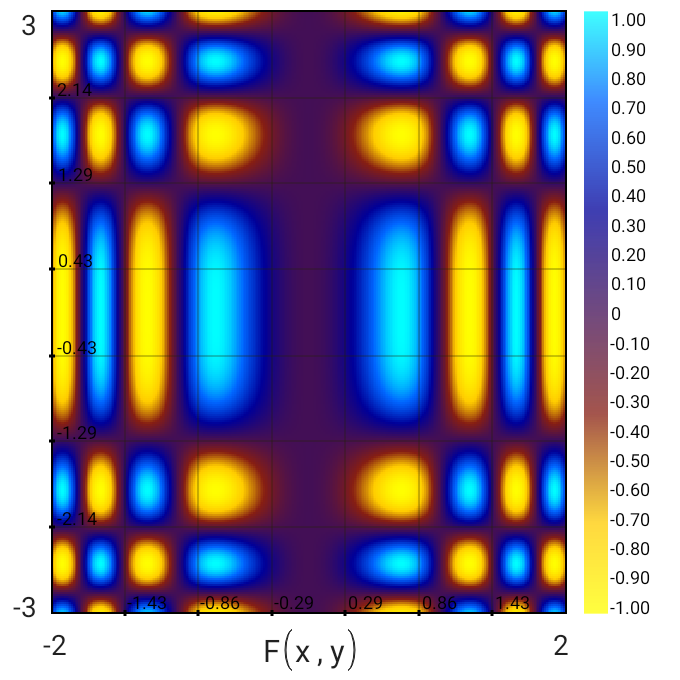
\includegraphics[resolution=320]{graphics/three_d_plot_fig2.png} \end{tabular}\end{center}

The plot boundaries, plot size and
style, labels and grid can be adjusted
by analogy with the function plot
using the plot settings dialog (see
''Function Plot'' example from the app
navigation drawer for more details).
To open this dialog, long click on the
plot area until the floating button
''Object properties'' will appear, and
than click this button.

Additionally, you can change the
number of labels along z-axis and
choose the color palette in the ''Color
Map Settings'' dialog. This dialog
appears by long click on the z-axis
bar on the right of main graph area.
\begin{center}\begin{tabular}{c}
  $R(x,y) := sin \left( 5 \cdot {x}^{2} \cdot \left( y - x \right)\right) $
\end{tabular}\end{center}
\begin{center}\begin{tabular}{c} 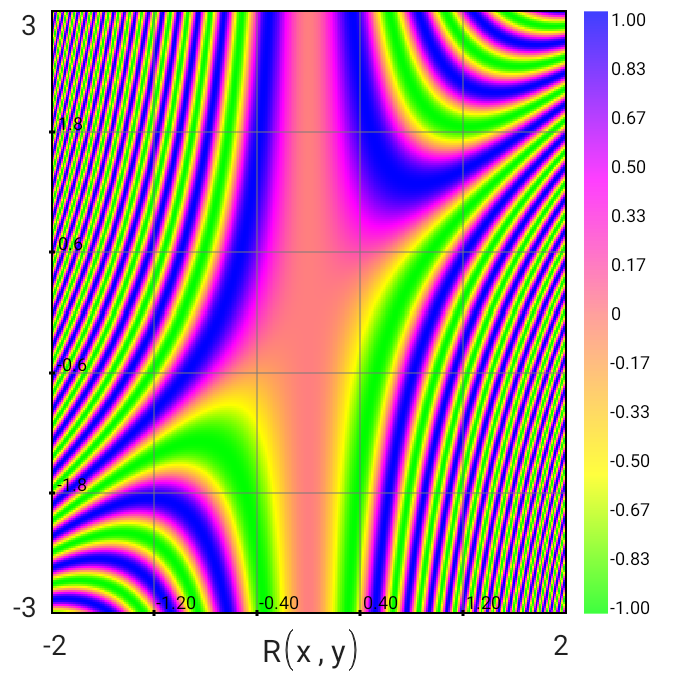
\includegraphics[resolution=320]{graphics/three_d_plot_fig3.png} \end{tabular}\end{center}

A function of two arguments can be also
plotted as a surface in 3D space. This
mode can be activated in the ''Plot
Settings'' dialog that appears if you
click floating button ''Object
properties'' after long clicking on the
plot area. Let us plot the following
function, using arrays in order to
improve calculation time:
\begin{center}\begin{tabular}{cccc}
  $N := 100$ &
  $n := \left[ 0,\, 1 \,..\, N \right]$ &
  $x1 := -15$ &
  $x2 := 15$ \cr
\end{tabular}\end{center}
\begin{center}\begin{tabular}{cccc}
  $M := 100$ &
  $m := \left[ 0,\, 1 \,..\, M \right]$ &
  $y1 := -15$ &
  $y2 := 15$ \cr
\end{tabular}\end{center}
\begin{center}\begin{tabular}{c}
  $x[n] := {\left( x1 +  \left( x2 - x1\right)  \cdot n / N \right)}^{2}$
\end{tabular}\end{center}
\begin{center}\begin{tabular}{c}
  $y[m] := {\left( y1 +  \left( y2 - y1\right)  \cdot m / M \right)}^{2}$
\end{tabular}\end{center}
\begin{center}\begin{tabular}{c}
  $r[n,m] := 0.04 \cdot x_{n}  + 0.02 \cdot y_{m} $
\end{tabular}\end{center}
\begin{center}\begin{tabular}{c}
  $t[n,m] := \left( x_{n}  + 0.05 \cdot y_{m}  \right) \cdot exp \left( 1 - r_{n,\, m} \right) $
\end{tabular}\end{center}
\begin{center}\begin{tabular}{c}
  $F[n,m] := \frac{sin \left( x_{n}  + 0.1 \cdot y_{m} \right) }{0.15 + r_{n,\, m} } + \frac{t_{n,\, m} }{10}$
\end{tabular}\end{center}
\begin{center}\begin{tabular}{c} 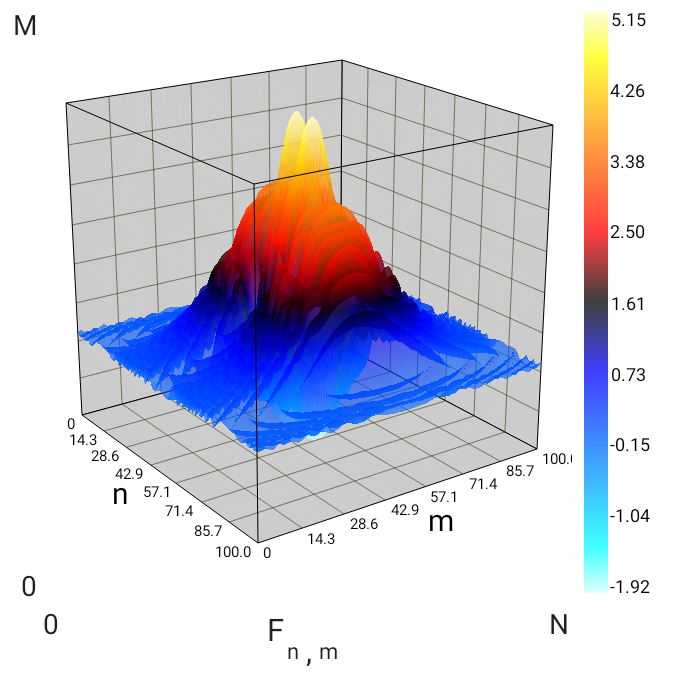
\includegraphics[resolution=320]{graphics/three_d_plot_fig4.png} \end{tabular}\end{center}

For the surface plot, there are
additional settings presented in the
''Plot Settings'' dialog. You can choose
whether the mesh lines shall be shown,
select the opacity for mesh color,
define the rotation and elevation
angles of the plot box. For example,
the previous surface plotted with
other rotation and elevation angles
looks like this: 
\begin{center}\begin{tabular}{c} 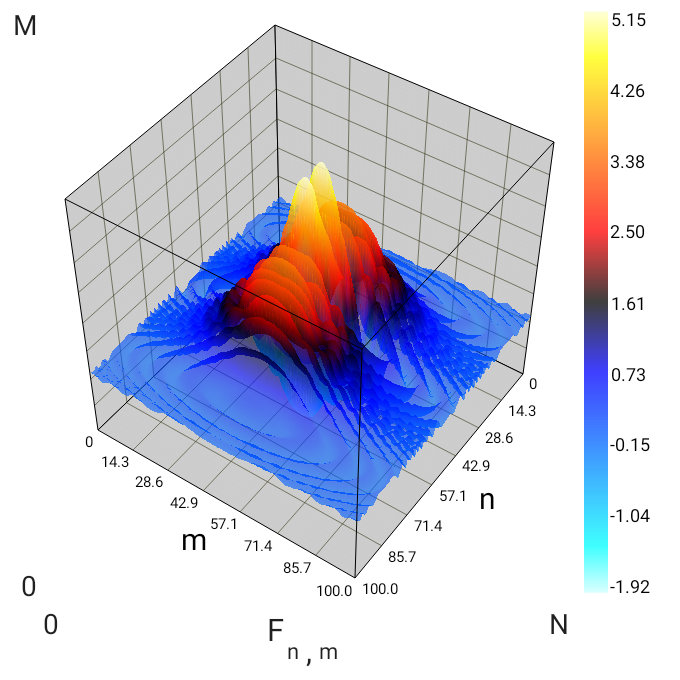
\includegraphics[resolution=320]{graphics/three_d_plot_fig5.png} \end{tabular}\end{center}